\subsection{La forza dell'aspettativa}

\begin{definition}[Aspettativa]
L'\textbf{aspettativa} è l'interpretazione che una persona dà prima che quel 
qualcosa accada. Tali aspettative influenzano la percezione della realtà di un 
individuo. 
\end{definition}

\begin{example}[Birra e aceto]
In un esperimento si son prese due caraffe di birra, contenenti 2 birre
differenti: una normale e una corretta con alcune gocce di aceto balsamico.
Ai soggetti (i normali avventori di un pub) veniva dato un assaggio di entrambe
poi un bicchiere della birra che preferivano.
I volontari dell'esperimento sono stati divisi in due gruppi: al primo gruppo
non venne spiegata la differenza tra le birre, mentre al secondo sì. I
risultati mostrarono che il primo gruppo scelse la birra con l'aceto, il
secondo la birra normale. Ciò è dovuto all'aspettativa: oggettivamente la birra
con l'aceto balsamico è buona, ma la nostra aspettativa ci induce a pensare che
non lo sia.

L'esperimento poi proseguì aggiungendo un terzo gruppo, al quale la
differenza tra le 2 caraffe di birra fu spiegata dopo l'assaggio, ma
prima della scelta e, anche in questo caso, la maggioranza scelse la birra
con l'aceto.

Tale esperimento dimostra quindi che l'aspettativa modifica
effettivamente la percezione del soggetto, lo stimolo gustativo stesso. 
\end{example}

L'aspettativa è una forma di pensiero definita di alto livello: quel qualcosa
viene interpretato qui e ora, e proiettata nel futuro. Questi livelli di
elaborazione nel cervello sono molto alti e sono in grado di influenzare
elementi informativi molto più bassi, tanto da arrivare a modificare elementi 
di percezione. Quindi se io creo delle aspettative su qualcosa, in qualsiasi 
modo questa venga fatta, si avranno della sensazioni diverse. Anche le 
etichette sui contenitori del cibo lavorano in questa maniera: più creano una 
buona aspettativa, più effettivamente una persona troverà tale pietanza buona!

Quando una aspettativa viene delusa si hanno delle grosse ripercussioni, anche
se, in generale, creare una buona aspettativa fa sì che un prodotto venga
considerato in maniera più positiva.

\begin{example}[Impiattamento]
Un esempio in cui l'aspettativa gioca un ruolo chiave è l'impiattamento.
Tutti noi preferiamo mangiare un piatto ben curato e questo perché altera la
nostra aspettativa: migliore sarà l'impiattamento, maggiore sarà la nostra
aspettativa, più la pietanza ci sembrerà buona. 
\end{example}

\begin{example}[Packaging]
Il \emph{packaging} di un bene si rivela essere importante: non si può 
insinuare che la confezione valga tanto come il prodotto al suo interno ma 
contribuisce alla soddisfazione dell'acquirente. Prodotti come i profumi spesso 
presentano boccette molto elaborate proprio per questo scopo. 
\end{example}

Tutto ciò ci insegna che il primo impatto e l'apparenza sono molto importanti,
e permette di influenzare la qualità del prodotto percepita dall'utente. Non
tutti ne sono influenzati allo stesso modo, ma nessuno ne è completamente
indifferente.

\subsection{La forza del brand}

Quanto arriva a essere potente la \textbf{forza di un brand}, non solo da un
punto di vista economico ma anche dal punto di vista dell'aspettativa?
Il brand, uno degli asset più significativi per un'azienda, si basa
pesantemente sull'aspettativa del cliente nei confronti di quella marca.

\begin{example}[Coca-cola vs Pepsi]
In un test d'esempio tra la Coca-cola e la Pepsi è stato utilizzato l'fRMI. In
un test cieco si attivano solo le aree deputate alla percezione gustativa e
molti soggetti finivano col preferire la Pepsi. Se i soggetti vengono
informati sulla bibita che stanno per assaggiare, si attivano anche altre
aree cerebrali, totalmente slegate al gusto, ma legate alle emozioni e ai
ricordi (come l'ippocampo e la corteccia prefrontale dorso laterale, facenti
parte del mid brain). Queste venivano attivate in quantità maggiore nel caso
della Coca-cola e, difatti, la maggior parte dei soggetti, in questo caso,
preferì quest'ultima. Sono questi processi cognitivi aggiuntivi che danno un
vantaggio di mercato alla Coca Cola, non le sue proprietà chimiche. 
\end{example}

Quando il brand è noto e si hanno alte aspettative si attivano tutta una serie
di processi cognitivi, che altrimenti non verrebbero attivati. Questa è la vera
potenza di un brand: se un marchio è in grado di attivare il nostro ippocampo
ed evocare emozioni e ricordi in noi vuol dire che può facilmente influenzare
le nostre decisioni.

Queste considerazioni non sono limitate agli oggetti e ai marchi, ma anche alle
persone. Anche per questo, negli ultimi anni, è nato il \textbf{self-branding}, 
a cui sono strettamente legate tutte le attività di
\textbf{self-promoting}.
\begin{definition}[Self-branding]
Per \textbf{self-branding} s'intende la gestione di sé stessi e della propria 
reputazione come se fosse un brand.
\end{definition}

Queste attività sono particolarmente importanti per 
consulenti, youtuber, politici, ecc\dots{}

\subsection{La reputazione}

Nel passato, gli acquisti di determinati prodotti costruiva attorno a un brand
una determinata reputazione. Con l'avvento della pubblicità di
massa\footnote{Detta anche pubblicità \textit{broadcast}. Nota: la sua
efficacia cala di anno in anno, in quanto l'utente è più informato rispetto al
passato, grazie soprattutto ad Internet.}, e con la popolazione non
adeguatamente informata, i brand potevano facilmente pubblicizzare
il loro prodotto come il migliore. Soprattutto grazie al Web 2.0 ora
è più facile per i consumatori diffondere la loro opinione ad altri su un
determinato prodotto, rendendo la vita più ``difficile'' ai brand. In questa
maniera i brand hanno bisogno di mantenere un'alta reputazione e devono
prestare attenzione alla comunicazione con gli utenti.

La \textbf{brand reputation} è la gestione della reputazione di un marchio, che
comprende anche il comportamento associato alle persone dell'azienda e la sua
presenza sui social.

\subsection{Gamification}

\begin{definition}[Gamification]
Con \textbf{gamification} si intende l'utilizzo di tecniche, regole e dinamiche
tipiche del mondo dei giochi in contesti diversi da quelli ludici.
Significa utilizzare meccaniche e dinamiche di gioco come punti, livelli,
reward, missioni e status all'interno di contesti non gaming per creare
engagement e risolvere problemi. 
\end{definition}

\noindent La gamification costituisce uno strumento in grado di agire 
visceralmente sugli istinti umani, spingendo spesso gli utenti, ora giocatori, a 
modificare le proprie abitudini all’interno di un sistema reso ``more fun''.

\begin{figure}[t]
 \centering
 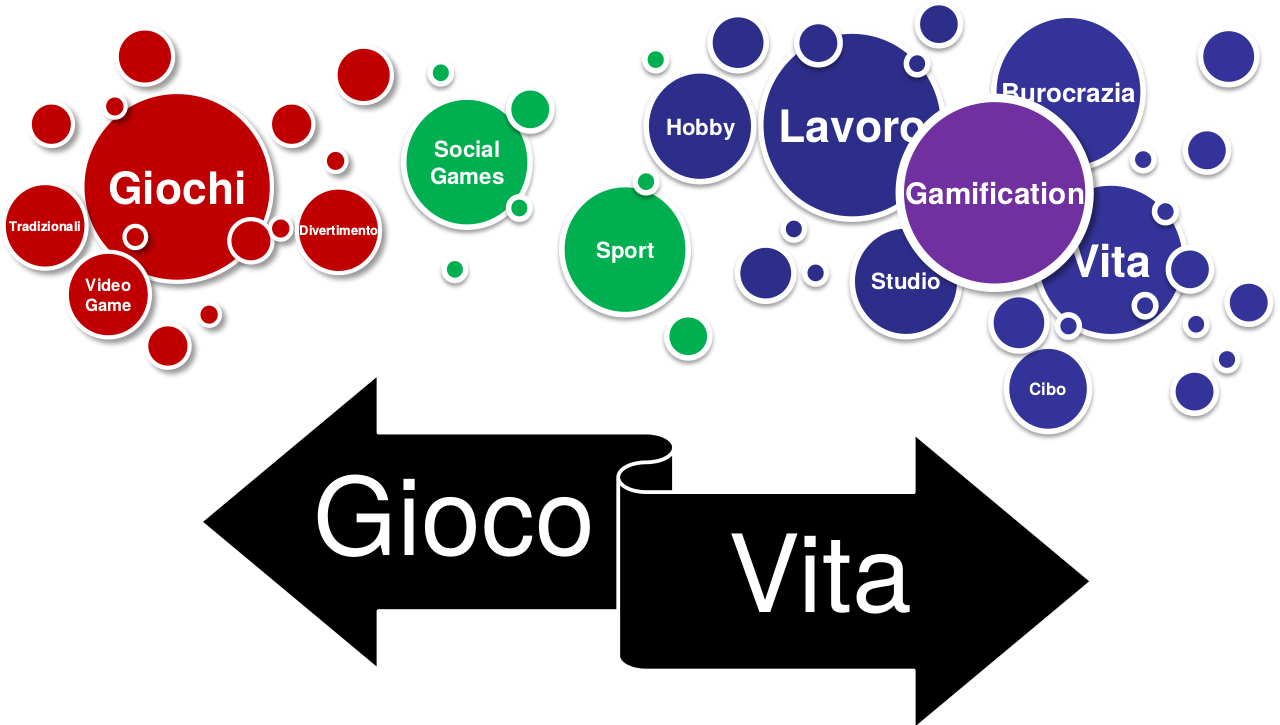
\includegraphics[scale=0.3]{gamification}
 \caption[Gamification]{Grafico degli universi in cui la gamification può 
essere applicata}
 \label{fig:neuro:gamification}
\end{figure}

Esistono diversi universi in cui questa tecnica viene impiegata, come 
mostrato in Figura~\ref{fig:neuro:gamification}. La gamification significa 
unire il gioco e divertimento con il resto degli universi. Attenzione! Non 
bisogna confondere \emph{gamification} e \emph{game design}. La 
\emph{gamification} infatti aggiunge meccaniche gaming su un prodotto pensato 
per finalità differenti, mentre il \textit{game design} si occupa di dar vita 
ad un gioco vero e proprio, un prodotto profondo ed immersivo che non risulti 
né troppo difficile né troppo complicato da imparare in modo di far si che 
l'utente utilizzi il gioco per il maggior tempo possibile senza annoiarsi.

In cosa può essere usata la gamification? Questa si differenzia dalla
pubblicità (pubblicizzo un mio prodotto) e dalla promozione (ad es. prendi 3
paghi 2, sorpresa negli oggetti che si comprano). Nella pubblicità, infatti, si
incentiva la brand awareness, ha bisogno di grossi investimenti e si hanno
guadagni a lungo termine: anche nel caso in cui si sospenda un determinato spot
pubblicitario i suoi effetti rimarranno per un determinato periodo di tempo. Le
promozioni, invece, non aumentano la brand awareness, ma incentivano
immediatamente le vendite per la durata della promozione stessa. La
gamification \emph{non} è una promozione, e coinvolge un sistema a
punteggio/livelli, a cui sono collegate solitamente delle \textbf{reward} e può 
avere un certo grado di competizione (con altri o con sé stessi).
La gamification è efficace perché è una tecnica forte per scardinare le
abitudini. Le abitudini sono dei comportamenti radicati nell'individuo,
difficili da modificare (ad esempio cambiare un'abitudine alimentare è
faticoso) poiché ci sarebbe un costo fisico o emotivo da pagare, anche se
razionalmente si sa che modificare una determinata abitudine potrebbe portare a
dei benefici. Questa tecnica funziona bene sopratutto nell'ambito delle diete e
del fitness. La capacità di questa tecnica di rompere le regole aggiunge una
variabile nella scelta compiuta da nostro cervello che non è più solamente tra
una gratificazione immediata (gestita dal mid brain) o a lungo termine 
ragionata e quindi che lavora sul new brain, che può essere per esempio la
gratificazione sociale (\emph{like} ai post, incitamento mentre si corre da
parte di altri utenti, \dots{}).

È importante nella vendita dei prodotti tenere conto di come funziona il nostro
cervello, quindi:

\begin{itemize}
 \item alcuni prodotti vengono scelti e valutati dalla nostra mente razionale
 (ad esempio le tariffe telefoniche);
 \item altri parlano con le nostre sensazioni e/o ricordi (trailer del cinema,
 cibo).
\end{itemize}

Le pubblicità devono parlare con le aree preposte del nostro cervello, cioè nel 
primo caso al new brain, nel secondo al mid brain. È importante \textbf{non 
mescolare} i diversi stili di comunicazione, in quanto prevale sempre la parte 
emozionale su quella razionale, poiché gli aspetti del mid brain sono più 
legati alla sopravvivenza o alla riproduzione. Non ha senso quindi 
sponsorizzare delle tariffe telefoniche con un/una bel/la ragazzo/a mezzo 
nudo/a poiché si deve parlare con la parte razionale e non emozionale.

Per riassumere, la gamification inserisce degli elementi di dialogo
con la mente emozionale.
